\documentclass[15pt]{report}

\usepackage{amssymb}
\usepackage{amsmath}
\usepackage{fp}
\usepackage{geometry}
\usepackage{graphicx}
\usepackage[utf8]{inputenc}
\usepackage{mathtools}
\usepackage{media9}
\usepackage{multicol}
\usepackage[parfill]{parskip}
\usepackage{pgfplots}
\usepackage{pstricks}
\usepackage{sectsty}
\usepackage[]{tikz}
\usepackage[pagestyles]{titlesec}
\usepackage{xcolor}
\usetikzlibrary{decorations.pathreplacing}
\usepackage{multirow,bigdelim}
\newenvironment{Table}
   {\par\bigskip\noindent\minipage{\columnwidth}\centering}
   {\endminipage\par\bigskip}
\usepackage{etoolbox}
\makeatletter
\patchcmd{\chapter}{\if@openright\cleardoublepage\else\clearpage\fi}{}{}{}
\makeatother

\definecolor{usm}{RGB}{176,153,40}
\chapterfont{\color{usm}}  % sets colour of chapters
\sectionfont{\color{usm}}  % sets colour of sections
\begin{filecontents}{timeline.txt}
::0x0 % coordinate system & y=e^x, repeated until last frame
::1 % one blue curve per frame
::2
::3
::4
::5
::6
::7
::8
\end{filecontents}

\headheight = -0.5cm
\oddsidemargin = 0cm % margen izquierdo 4.5-2=2.5cm
\pgfplotsset{compat=1.7}
\textheight = 23.5cm % largo texto impreso
\textwidth = 18cm % ancho texto impreso
\titleformat{\chapter}[display]
  {\normalfont \bfseries}{}{0pt}{\Large}
\topmargin = -2cm % margen superior 3-2=1cm

%RENAME
\renewcommand{\chaptername}{\underline{Capítulo}}
\renewcommand{\contentsname}{\color{usm}\underline{\textbf{CONTENIDO}}}
\renewcommand{\figurename}{Figura}
\renewcommand{\tablename}{Tabla}

\title{
        {\sc \bf \color{usm} \huge{COSTOS}\\ \LARGE{plaje}}
        \\
%        {\vfill}
%       \\
      {\includegraphics[scale=0.17]{unmsm.png}}
       \\
        {Rufasto C. Andy}
       \\
        {Facultad de Ciencias Económicas}
       }
    \author{RUFASTO C. ANDY}
    \date{}

\begin{document}
	\begingroup
	\Large
	\maketitle 
\newpage
	\tableofcontents
\newpage
	\chapter{\color{usm}Costos}
	\maketitle \vskip-25pt \hrule\vskip10pt
\section{Definición}
	Es el proceso de medir, analizar, calcular e informar sobre el costo, la rentabilidad y la ejecución  de las operaciones de la empresa.

\section{Objetivos}
	\begin{itemize}
\item Ayudar a la empresa a la toma de decisiones correctas.\\
\item Evaluar la actividad de la empresa.\\
\item Medir el resultado economico.\\
\end{itemize}

\newpage
	\chapter{\color{usm}Tipos de Coste}
	\maketitle \vskip-25pt \hrule\vskip10pt
	\[
\text{Tiempo}
\begin{cases}
Histórico \\ Futuro
\end{cases}
\]

\[
\text{Unidad de Referencia}
\begin{cases}
Directo \\ Indirecto
\end{cases}
\]

\[
\text{Volumen}
\begin{cases}
Fijo \\ Variable
\end{cases}
\]

\[
\text{Nivel de producción}
\begin{cases}
Unitarias \\ Totales
\end{cases}
\]


	\endgroup
	\chapter{\color{usm}Costo Absorvente}
	\begin{Large}

\begin{multicols}{3}

\begin{Table}
\begin{tabular}{rll}
 & IIMP &  \\
+ & Comp &  \\ \hline
 & MPD  &  \\
- & IFMP &  \\ \hline
 & MP   & 
\end{tabular}
\end{Table}

\columnbreak
	
\begin{Table}
\begin{tabular}{lll}
  & MP   &  \\
+ & MOD  &  \\
+ & GGF  &  \\ \hline
  & CFAB &  \\
+ & IIPP &  \\
- & IFPP &  \\ \hline
  & CMM  &  \\
+ & IIPT &  \\
- & IFPT &  \\ \hline
  & CMV   & 
\end{tabular}
\end{Table}

\columnbreak
\begin{Table}
\begin{tabular}{lll}
  & IV    &  \\
- & CMV   &  \\ \hline
  & UB    &  \\
- & GP    &  \\ \hline
  & Uop   &  \\
  & ING   &  \\ \hline
  & UAI   &  \\
- & INP   &  \\ \hline
  & UN    &  \\
- & DIV   &  \\ \hline
  & U.RET & 
\end{tabular}
\end{Table}

\end{multicols}

\end{Large}


	\chapter{\color{usm}Costo Variable o Directo}
	
\begin{table}[h]
\Large
\center
	\begin{tabular}{rc}
	 & IV \\
	- & CV \\ \hline
	& Mc	\\
	-& CF	\\ \hline
	& U,OP \\
	& \vdots
	\end{tabular}
\end{table}



\newpage
	\chapter{\color{usm}Costos por Proceso}
	\section{Promedio}

\begin{table}[h]
\centering
\begin{tabular}{lrl}
+ & IIPP          &  \rdelim\}{4}{mm}[Flujo de Unidades] \\
+ & U. emp        &  \\ \cline{1-2}
  & U. Disp       &  \\
- & IFPP          &  \\ \cline{1-2}
  & U. Trans      &  \rdelim\}{3}{mm}[Unidades Equivalentes] \\
+ & U IFPP (\% A) &  \\ \cline{1-2}
  & U Eq          & 
\end{tabular}
\end{table}
\centering
\[
\hspace{1.4cm}
\begin{rcases*}
CF_{ EyT }=\dfrac{ C.\: inc + C.\; agr }{ Ueq } \\ 
CF_{IFPP}=CF_{EyT} \times (\%A) 
\end{rcases*} \text{Calculo CF} 
\]
\begin{table}[h]
\hspace{1.9cm}
\begin{tabular}{llll}
+ & U. EyT \times CF_{EyT}       & = CT_{EyT}    &  \rdelim\}{3}{mm}[Informe de Costos]\\
+ & U. IIPPyT \times  CF_{IIPPyT} & = CT_{IIPPyT} &  \\ \cline{2-3}
  & Costos Transferidos                            & = C. agr + C. inc  & 
\end{tabular}
\end{table}

\begin{table}[h]
\hspace{0.9cm}
\begin{tabular}{lllllllll}
\multicolumn{2}{l}{Costos Varios} &  & \multicolumn{2}{l}{Inv. P. Proc}              &  & \multicolumn{2}{l}{Inv. P. Term}        &  \rdelim\}{3}{mm}[Registro Contable]  \\ \cline{1-2} \cline{4-5} \cline{7-8} 
\multicolumn{1}{l|}{}   & C. inc  &  & \multicolumn{1}{l|}{C. inc} & CT_{U. Tran} &  & \multicolumn{1}{l|}{CT_{U. Tran}} &  &  \\
\multicolumn{1}{l|}{}   & C. agr  &  & \multicolumn{1}{l|}{C. agr} &                 &  & \multicolumn{1}{l|}{}                &  & 
\end{tabular}
\end{table}
\newpage

\section{Fifo}

\begin{table}[h]
\centering
\begin{tabular}{lrl}
+ & IIPP          &  \rdelim\}{4}{mm}[Flujo de Unidades] \\
+ & U. emp        &  \\ \cline{1-2}
  & U. Disp       &  \\
- & IFPP          &  \\ \cline{1-2}
  & U. Trans      &  \rdelim\}{5}{mm}[Unidades Equivalentes] \\
- & U. IIPP        &  \\
+ & U. IIPP (\% F) & \\
+ & U IFPP (\% A) &  \\ \cline{1-2}
  & U Eq          & 
\end{tabular}
\end{table}
\centering
\[
\hspace{cm}
\begin{rcases*}
CF_{ EyT }=\dfrac{C.\; agr }{ Ueq } \\ 
CF_{IFPPyT}= \dfrac{C.\;inc }{ U. IIPP} + CF_{EyT}(\% F)\\
CF_{IFPP}= CF_{EyT}(\% A)
\end{rcases*} \text{Calculo CF} 
\]
\begin{table}[h]
\hspace{1.9cm}
\begin{tabular}{llll}
+ & U. EyT \times CF_{EyT}       & = CT_{EyT}    &  \rdelim\}{3}{mm}[Informe de Costos]\\
+ & U. IIPPyT \times  CF_{IIPPyT} & = CT_{IIPPyT} &  \\ 
+ & U IFPP \times CF_{IFPP} & = CT_{IFPP} & \\ \cline{2-3}
  & Costos Transferidos                            & = C. agr + C. inc  & 
\end{tabular}
\end{table}

\begin{table}[h]
\hspace{0.9cm}
\begin{tabular}{lllllllll}
\multicolumn{2}{l}{Costos Varios} &  & \multicolumn{2}{l}{Inv. P. Proc}              &  & \multicolumn{2}{l}{Inv. P. Term}        &  \rdelim\}{3}{mm}[Registro Contable]  \\ \cline{1-2} \cline{4-5} \cline{7-8} 
\multicolumn{1}{l|}{}   & C. inc  &  & \multicolumn{1}{l|}{C. inc} & CT_{U. Tran} &  & \multicolumn{1}{l|}{CT_{U. Tran}} &  &  \\
\multicolumn{1}{l|}{}   & C. agr  &  & \multicolumn{1}{l|}{C. agr} &                 &  & \multicolumn{1}{l|}{}                &  & 
\end{tabular}
\end{table}

	\flushleft
	\chapter{\color{usm}Costos Estándar}
	\section{Materia Prima}

\begin{equation*}
\centering
   Desv. \; Eficiencia + Desv. \; Precio  = Desviacion \; Contable
\end{equation*}

\tikzset{every picture/.style={line width=0.75pt}} %set default line width to 0.75pt        

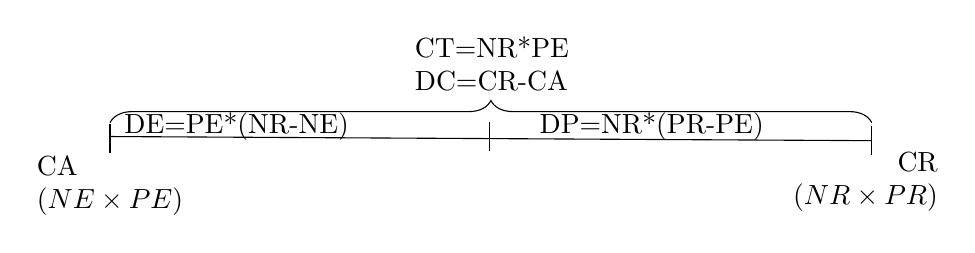
\begin{tikzpicture}[x=0.75pt,y=0.75pt,yscale=-1,xscale=1]
\centering

\draw    (94,110) -- (461,112) ;
\draw    (94,104) -- (94,118) ;
\draw    (277,103) -- (277,117) ;
\draw    (461,105) -- (461,119) ;
\draw[decorate, decoration = {brace, amplitude = 8pt}, xshift = 0pt, yshift = 10pt] (94, 90) -- (461, 90);
\draw (458,132) node  [align=right] {CR \\ ($NR \times PR$)};
\draw (94,134) node  [align=left] {CA \\ ($NE \times PE$)};
\draw (278,75) node  [align=left] {CT=NR*PE \\ DC=CR-CA};
\draw (355,105) node  [align=left] {DP=NR*(PR-PE)};
\draw (155,105) node  [align=left] {DE=PE*(NR-NE)};

\end{tikzpicture}

\section{Mano de Obra}

\begin{equation*}
\centering
   Desv. \; Eficiencia + Desv. \; Tasa \; Salarial  = Desviacion \; Contable
\end{equation*}

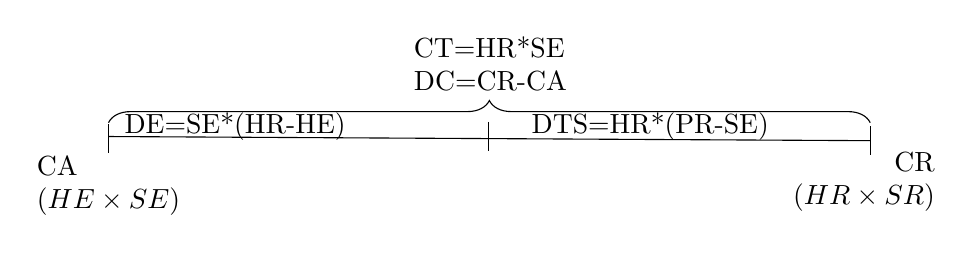
\begin{tikzpicture}[x=0.75pt,y=0.75pt,yscale=-1,xscale=1]
\centering

\draw    (94,110) -- (461,112) ;
\draw    (94,104) -- (94,118) ;
\draw    (277,103) -- (277,117) ;
\draw    (461,105) -- (461,119) ;
\draw[decorate, decoration = {brace, amplitude = 8pt}, xshift = 0pt, yshift = 10pt] (94, 90) -- (461, 90);
\draw (458,132) node  [align=right] {CR \\ ($HR \times SR$)};
\draw (94,134) node  [align=left] {CA \\ ($HE \times SE$)};
\draw (278,75) node  [align=left] {CT=HR*SE \\ DC=CR-CA};
\draw (355,105) node  [align=left] {DTS=HR*(PR-SE)};
\draw (155,105) node  [align=left] {DE=SE*(HR-HE)};

\end{tikzpicture}

	\chapter{\color{usm}Presupuesto}
	\Large
Plan contable en el que se definen las ventas que se tienen  que alcanzar en un futuro.\\
\begin{itemize}
\item Pan Contable Recoge información la ordena, clasifica y resume.\\
\item \textbf{Metas económicas} en términos totales.\\
\item \textbf{Proyección al futuro}.\\
\item \textbf{Balance proyectado}.\\
\item \textbf{Estado de ganancias y pérdidas proyectado}.\\
\end{itemize}


\end{document}


